\section{Learning Rectangle Problem using SQ}
\label{sec:implementation}

In this section, we implement an algorithm to learn the rectangle problem introduced in \cite{blumer_learnability_1989} using a statistical query oracle. The objective is to learn an unknown axis-aligned target rectangle $R$ which forms the boundary between a set of points in the Euclidean plane $\R^2$. The points inside the rectangle are positive examples and the ones outside are negative. Figure \ref{fig:rectangle_problem} shows the target rectangle $R$ along with a sample of positive and negative examples.

\begin{figure}
    \centering
    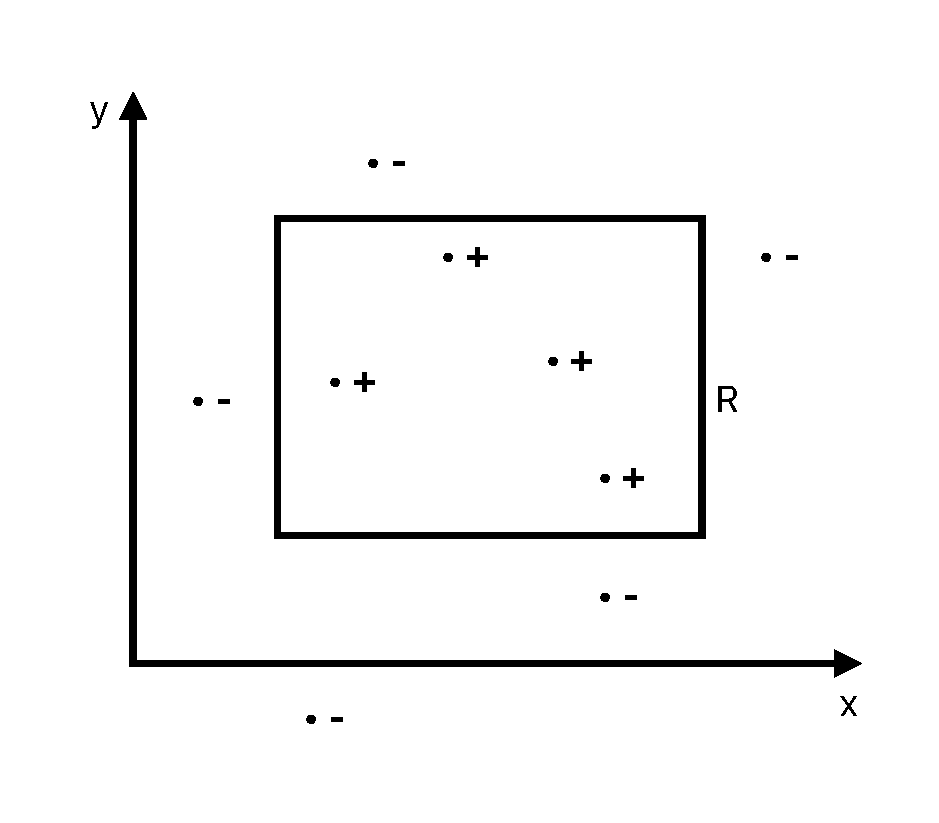
\includegraphics[width=0.36\textwidth]{report/figs/Rectangle.pdf}
    \caption{The target rectangle $R$ along with a sample of positive and negative examples \cite{kearns_introduction_1994}}
    \label{fig:rectangle_problem}
\end{figure}

To solve this problem using the statistical query learning framework, first, we define our concept class $C: \R^2 \xrightarrow{} \{-1, 1\}$, the statistical query $\chi: \R^2 \times \{-1, 1\} \xrightarrow{} \{-1, 1\}$ and the statistical query oracle $SQ(c, \cD)$. The statistical query oracle when given a function $c \in C$, will return an estimate of the expectation of whether the current hypothesis rectangle is correctly separating the positive and negative points $\nu: |\nu - \mathbb{E}_{\cD}[\chi(x, c(x))]| \leq \tau$. Now, we propose an algorithm to solve this problem using the defined statistical query oracle.

\begin{algorithm}[!h]
\caption{Rectangle Problem using SQ}
\label{rectangle_algo}
\begin{algorithmic}[1]
% \State $i \gets 10$
\State Input $SQ, \epsilon, min, max, \delta$
\State Initialize $c$ randomly to be a valid rectangle
\State Initialize $\nu \gets \infty, \Delta, c'$
\While{$|1 - \nu| > \epsilon$}
    \State $\Delta \gets Random(min, max, (max-min)*\delta)$
    \State $c' \gets c$
    \If{$Random(0, 1) < 0.5$}
        \State Change lower-left point by of $c'$ by $\Delta$
    \Else
        \State Change upper-right point of $c'$ by $\Delta$
    \EndIf
    \If{$c'$ is not valid}
        \State Skip to next iteration
    \EndIf
    % \If{$Random(0, 1) < 0.5$}
    %     \If{$Random(0, 1) < 0.5$}
    %         \State Increase $c'$ along x-axis by $w.\delta$
    %     \Else
    %         \State Decrease $c'$ along x-axis by $w.\delta$
    %     \EndIf
    % \Else
    %     \If{$Random(0, 1) < 0.5$}
    %         \State Increase $c'$ along y-axis by $w.\delta$
    %     \Else
    %         \State Decrease $c'$ along y-axis by $w.\delta$
    %     \EndIf
    % \EndIf
    \State $\nu' \gets SQ(c')$
    \If{$|1-\nu'| < |1-\nu|$}
        \State $\nu \gets \nu'$
        \State $c \gets c'$
    \EndIf
\EndWhile
\State Output $c$
\end{algorithmic}    
\end{algorithm}

\subsection{Algorithm}

Since each valid rectangle can be represented by two points, the lower-left point and the upper-right point, Algorithm \ref{rectangle_algo} changes either of these with equal probability. The change is based on some hyperparameters of the algorithm, $\epsilon, min, max \text{ and } \delta$. $\epsilon$ is the maximum error of the resultant hypothesis. $min \text{ and } max$ describe the minimum and maximum value we can take along the two axes. There is also another hyperparameter $\tau$ which is part of the statistical query oracle and it defines how close the estimate provided by the oracle is to the true value. The $Random$ function of Line 5 gives a random number in the range defined by $min \text{ and } max$ with the step size of $(max-min)*\delta$. To check whether a rectangle $c'$ is valid (Line 11), we check whether the points are in the range defined by $min \text{ and } max$, and if the values of the upper-right point along both the axes are greater than the lower-left point.

% Algorithm \ref{rectangle_algo} changes either of the two axes of the rectangle by a small value. It then checks with the statistical query oracle to see if the new rectangle estimate is better than the previous estimate. It loops through this process until the error of our rectangle estimate is better than $\epsilon$.

\subsection{Analysis}
\label{algo_analysis}
Algorithm \ref{rectangle_algo} does a random search over all the possible axis-aligned rectangles in the constraints defined by $min, max \text{ and } \delta$. In this section, we find an estimate of the number of these rectangles which is equal to the worst-case number of queries to the oracle. The region defined by these constraints will have roughly $\frac{1}{\delta^2}$ number of points from which we can choose the two points for a valid rectangle. The upper bound on the number of rectangles in this region can be given by $^{\frac{1}{\delta^2}}C_2 = \frac{1-\delta^2}{2.\delta^4} = O(\delta^{-4})$. Section \ref{app:algo_analysis} contains some results on the experiments conducted using the proposed algorithm.
